As an example of how to best employ the features of the DVFS plugin we have chosen the SeisSol application \cite{SeisSol} as our use case here. The SeisSol application is developed by the Department of Earth and Environmental Sciences at the Ludwig-Maximilian University. It is a MPI application written in Fortran 90. The application is used for simulating realistic earthquake scenarios, accounting for a variety of geophysical processes that affect the propagation of seismic waves, e.g. viscoelastic attenuation, strong material heterogeneities and anisotropy. SeisSol contains a computation kernel which simulates the specified number of time steps.

\subsubsection{Extending the search space}

The objective of the DVFS plugin is to tune the energy consumption of an application. The DVFS plugin can be configured with the number of frequencies that the plugin should use for the search space. The models predict one frequency according to the tuning objective. The number of neighboring frequencies (neighbors of the predicted frequencies) to be analyzed can be set. Environment variable PSC\_FREQ\_NEIGHBORS is used for this purpose. The value of this variable specifies the number of neighbors to the right and to the left of the predicted frequency. The maximum value for this variable is limited to 7 neighbors. If the value exceeds 7 neighbors or if it is negative then the plugin will use the default value of 1 neighbor on each side. The user is advised to use a higher number of neighbors when the execution time does not play a role, i.e., when the tuning is completed in an acceptable time-frame for the user. If it is suspected that the model delivers inaccurate predictions, a higher number of frequencies can help mitigate this problem.

Figure \ref{fig:seissol_dvfs_3_nebr} shows the sample output of the DVFS plugin for the SeisSol application with PSC\_FREQ\_NEIGHBORS=3. The tuning objective was to minimize the Energy Delay Product (EDP). 

\begin{figure}[H]
  \centering
  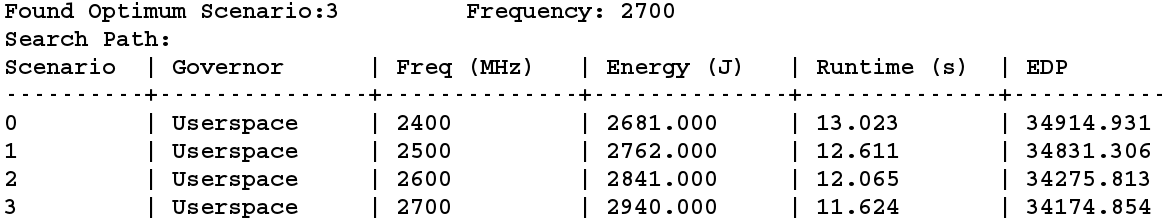
\includegraphics[scale=0.6, width=\textwidth]{../BPG/images/seissol_dvfs_3_nebr.png}
  \caption{Output of the DVFS plugin for inspecting the predicted and three neighbor frequencies.}
  \label{fig:seissol_dvfs_3_nebr}
\end{figure}

The output shows that the three neighbors below the predicted CPU frequency of 2.7\,GHz are measured compared to the default of one neighbor as shown in Figure\ref{fig:uc3_dvfs_model_3_results}. Since 2.7GHz is the highest CPU frequency supported by the Sandy Bridge processors of SuperMUC, only the three lower neighboring frequencies are evaluated. 

\subsubsection{Selection of phase regions}

There are several methods to prepare the application selected for energy tuning. Many scientific codes have a time stepping loop, also known as a phase region. The most common method is to target the phase region in a code for tuning. The phase region is typically the region that consumes the most amount of time. Instrumenting the phase region consists of simply inserting the appropriate directives as follows:

\begin{itemize}
		\item Fortran: \\
		DO i = 1, 10 \\
		!\$ MON USER REGION \\
		kernel... \\
		!\$ MON END USER REGION \\
		ENDDO !Instrumented var \\
		\item C/C++ \\
		for(int i = 0; i \textless 10; i++) \\
		\{ \\
		\#pragma start\_user\_region \\
		kernel... \\
		\#pragma end\_user\_region \\
		\} \\		
\end{itemize}

Not every application has an outermost iterative loop with a time stepping scheme that can be used as a phase region. Either the main region can be used as phase region, resulting in an automatic restart of the application for each experiment, or some other region can be marked a phase region to restrict the tuning to this region. 

PTF user region can also be used to mark code regions also for other purposes then as a phase region. If a single user region is given, this is assumed to be used as phase region in PTF. If multiple user regions are given, the phase region can be identified by an input argument to the PTF frontend. The argument has the format {\tt--phase=``\textless file id \textgreater:\textless region first line \textgreater ''}. For example: 

\begin{verbatim}
    psc\_frontend --apprun="./Seissolxx PAR.par" --mpinumprocs=32 
                  --tune=dvfs --phase="31:809" --sir=SeisSol.sir
\end{verbatim}


If there is no phase region use the command as you would normally do.

Note that there can only be one phase region within the source code and it should be the outer most loop of all other instrumented regions. The presence of phase regions ensure faster automatic tuning, as each experiment is carried out by running one iteration (as opposed to running the entire application per experiment).  It is important not to have significant variations of time among iterations, otherwise the comparisons between experiments will produce wrong results. If the iterations at the phase region are suspected to have variations among them, then do not use a phase region. The loop of the phase region should have at least $2m+1$ iterations, where $m$ is the number of frequencies chosen. One iteration is for the pre-analysis, and $2m$ other iterations for the experiments.

\subsubsection{Multiple tuning objectives}

There are three models used in this plugin to predict the best frequency for a given objective, i.e., one for each of the quantities  \textit{Time}, \textit{Power}, and \textit{Energy}. The rest of the models are derived from these three main models and are used for the tuning objectives. Energy is modeled directly and this is the default model of the DVFS Plugin. Nevertheless, there is an energy model derived from the product of modeled power and time separately (export the environment variable ``export PSC\_DVFS\_MODEL=2'' before running). Variations are not significant between these two energy models and the user is encouraged to use any of the two when tuning for energy consumption.

There are several tuning objectives that can be chosen. You can optimize the energy consumption, the energy delay product, tune for power capping, optimize the total cost of ownership, or tune the energy consumption for an allowed performance degradation. The choice of the metric depends on the needs of the user. Here are some examples:

\begin{itemize}

\item  Consider optimizing the energy consumption when other costs related to time are minimal compared to energy costs. (PSC\_DVFS\_MODEL is either 1 or 2)

\item The energy delay product provides a strong emphasis on time (export PSC\_DVFS\_MODEL=3). The formula has time squared times power.

\item Consider using the total cost of ownership when you need to balance the influence of power-related costs and time-related costs (export PSC\_DVFS\_MODEL=4).

The Total Cost of Ownership (TCO) was used with the following cost formula (given per compute node):

\begin{equation}\label{eq: TCO}
		  TCO = a \cdot P \cdot t + b \cdot t,
\end{equation}

where $P$ is the average power in watts, $t$ the time in seconds, $a$ the cost of the energy  (in the plugin $ a = 2.7 \cdot 10^{-4} [EUR/J]$), $b$ the cost of personnel and other fixed costs amortized over the lifespan of the HPC system (in the plugin $ b = 0.1115 [EUR/s] $).

\item Power capping is used to limit the power and avoid trespassing a system-wide power limit which can generate more costs as electric companies penalize strong oscillations (export PSC\_DVFS\_MODEL=5). The power capping tuning objective uses a maximum power limit of 110 W per node.\\

\item Use PSC\_DVFS\_MODEL=6 when the increase of performance should be greater than an increase in energy  consumption in order to choose higher frequencies and power capping is not needed.

\item Use PSC\_DVFS\_MODEL=7 when the increase of performance should be greater than the increase in power. This case is more restrictive than the previous policy (selected using PSC\_DVFS\_MODEL=6) as it considers power instead of energy.

\item Use PSC\_DVFS\_MODEL=8 when power capping considerations are important. The frequency used will be chosen such that the power used is below the power threshold or have significant performance increase with respect to the nominal frequency 2.0\,GHz.

\item Use PSC\_DVFS\_MODEL=9 when the performance degradation with respect to the nominal frequency should be no more than 10\%.

\end{itemize}
	
Figure \ref{fig:uc2_dvfs_result} shows the execution of the SeisSol application using a default energy model PSC\_DVFS\_MODEL=1 and thus tuning for minimum energy usage. 
	
\begin{figure}[H]
	\centering
	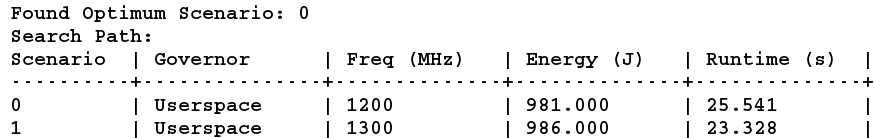
\includegraphics[scale=0.65]{../BPG/images/uc2_dvfs_result.png}
	\caption{Output of the DVFS plugin for energy tuning for SeisSol.}
	\label{fig:uc2_dvfs_result}
\end{figure}

The results show that executing SeisSol at 1.2 GHz would minimize the energy consumed during the execution. When choosing the Energy Delay Product as tuning objective instead of consumed energy, the plugin determines 2.6 GHz as the optimal frequency (Figure \ref{fig:uc3_dvfs_model_3_results}).

\begin{figure}[H]
	\centering
	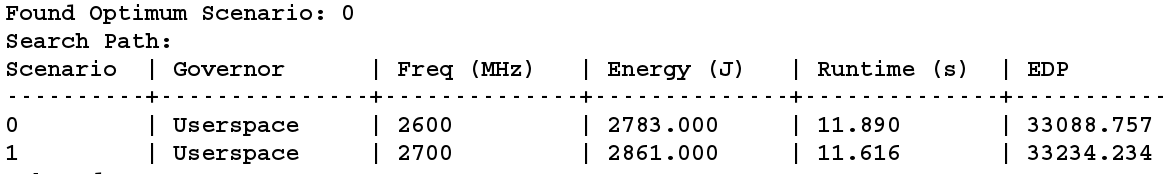
\includegraphics[scale=0.65, width=\textwidth]{../BPG/images/uc3_dvfs_model_3_results.png}
	\caption{Output of the DVFS plugin for tuning the Energy Delay Product for SeisSol.}
	\label{fig:uc3_dvfs_model_3_results}
\end{figure}


\subsubsection{Multiple application regions}

The DVFS plugin can not only determine a global best frequency but also individual best frequencies for different regions of the application. These regions have to be suited for energy tuning, i.e., they have to be coarse enough to amortize for the overhead of changing the processor frequency. 

To demonstrate this feature, three regions were marked in SeisSol for energy tuning. Table~\ref{table:regions}. The two inner regions group similar computations and are included in the phase region (region in calc\_seissol.f90). (In the table each region is given an identification number.)

\begin{table}[htpbH]
\centering
\begin{tabular}{|l|l|l|}
\hline
File & Region First Line & Region ID\\\hline
calc\_seissol.f90 & 489 & 1\\
galerkin3d\_tetra.f90 & 193 & 2 \\
galerkin3d\_tetra.f90 & 289 & 3\\\hline
\end{tabular}
	\caption{Instrumented regions in SeisSol.}
	\label{table:regions}
\end{table}

Tables~\ref{table:calcseis},~\ref{table:galerking3d1}, and~\ref{table:galerking3d2} show the results of for the SeisSol application when run with the tuning objective that optimizes
for energy consumption. Regardless of the tuning objective, the output of the plugin always displays the energy consumption, the runtime, Energy Delay Product ($EDP$), Energy Delay squared Product ($ED^2P$), the average power, and Total Cost of Ownership (TCO). Time and energy (and indirectly average power) are measured and reported on in the output.

\begin{table}[htpbH]
\centering
\begin{tabular}{|c |c |c |c |c |c |c|}
\hline
Frequency & Energy & Runtime & EDP           & EDDP            & Average Power & TCO \\
~[GHz]  & [$J$]  & [$s$]   &  [$J\cdot s$] & [$J\cdot s^2$]  & [Watt]        & [Euro] \\
\hline\hline
1.6       & 1132   & 18.196  & 20597.4    & 374782.4  & 62.2       & 2.3341\\
1.7       & 1143   & 17.075  & 19516.6    & 333244.2  & 66.9       & 2.2121\\
1.8       & 1172   & 16.230  & 19021.3    & 308712.3  & 72.2       & 2.1257\\
\hline
\end{tabular}
	\caption{Energy figures for Region~1.}
	\label{table:calcseis}
\end{table}

\begin{table}[htpbH]
\centering
\begin{tabular}{|c |c |c |c |c |c |c|}
\hline
Frequency & Energy & Runtime & EDP          & EDDP      & Average Power & TCO \\
~[GHz]  & [J]  & [s]   & [J$\cdot$ s] & [$Js^2$]  & [Watt]        & [Euro] \\
\hline\hline
1.6       & 185   & 1.545  & 285.8    & 441.6  & 119.7       & 0.2222\\
1.7       & 185   & 1.548  & 286.4    & 443.5  & 119.5       & 0.2226\\
1.8       & 186   & 1.547  & 287.8    & 445.4  & 120.2       & 0.2227\\
\hline
\end{tabular}
	\caption{Energy figures for Region~2.}
	\label{table:galerking3d1}
\end{table}

\begin{table}[H]
\centering
\begin{tabular}{|c |c |c |c |c |c |c|}
\hline
Frequency & Energy & Runtime & EDP          & EDDP      & Average Power & TCO \\
~[GHz]  & [J]  & [s]   & [J$\cdot$ s] & [$Js^2$]  & [Watt]        & [Euro] \\
\hline\hline
1.6       & 912   & 16.2  & 14805.2  & 240345.1 & 56.2       & 2.0560\\
1.7       & 928   & 15.3  & 14152.7  & 215837.8 & 60.8       & 1.9507\\
1.8       & 971   & 14.6  & 14136.7  & 205814.7 & 66.7       & 1.8852\\
\hline
\end{tabular}
	\caption{Energy figures for Region~3.}
	\label{table:galerking3d2}
\end{table}

These results show that using 1.6\,GHz optimizes the energy consumption of SeisSol for all three regions. The energy savings per region with respect to the worst case scenario are shown in Table~\ref{table:regionsavings}.

\begin{table}[H]
 \centering
 \begin{tabular}{| c | c | }
  \hline
  Region ID & Energy Savings \\\hline\hline
      1     &  3.4\%         \\\hline
      2     &  0.5\%    \\\hline
      3     &  6.1\%	\\
  \hline
 \end{tabular}
 \caption{Energy savings per region.}
 \label{table:regionsavings}
\end{table}

The plugin can be configured to use a tuning objective of either EDP, power capping, or TCO.  The EDP search space is the same as the one shown in Tables~\ref{table:calcseis}, \ref{table:galerking3d1}, and~\ref{table:galerking3d2}. The results for the case of EDP point to an optimization when using 1.8\,GHz for the outer loop (Region 1) and Region 3. The frequency that tunes EDP for Region 2 is 1.6 GHz.

The results of the tested scenarios for TCO are shown in Table~\ref{table:seissol_tco}. The minimum TCO is achieved by setting 2.7 GHz and costs are reduced by 2.3\%.

\begin{table}[H]
\centering
\begin{tabular}{|c |c|}
\hline
Frequency & TCO \\
~[GHz]  & [Euro] \\
\hline\hline
2.6       & 1.7438 \\
2.7       & 1.7055 \\
\hline
\end{tabular}
	\caption{DVFS output for Region 1 for TCO.}
	\label{table:seissol_tco}
\end{table}

\subsubsection{Automatic implementation of the advice}

The output of the DVFS plugin is not only printed to standard out, but also given in a special formatted file for the enopt library. The instrumented application can be linked exclusively with enopt (without PTF) for production runs. In this case, the enopt library will read the region-specific settings from the output file and automatically enforce them at runtime.


